\section{AES} \label{sec:AES}
AES is based on a design principle known as a substitution–permutation network, and is efficient in both software and hardware.
\\
\\
\textbf{High-level description of the algorithm}:
\begin{enumerate}
	\item KeyExpantion: round keys are derived from the cipher key using Rijndael's key schedule. AES requires a separate 128-bit round key block for each round plus one more.
	\item Initial round key addition:
		\begin{enumerate}
			\item AddRoundKey: each byte of the state is combined with a block of the round key using bitwise xor.
		\end{enumerate}
	\item For 9, 11 or 13 rounds:
		\begin{enumerate}
			\item SubBytes: a non-linear substitution step where each byte is replaced with another according to a lookup table.
			\item ShiftRows: a transposition step where the last three rows of the state are shifted cyclically a certain number of steps.
			\item MixColumns: a linear mixing operation which operates on the columns of the state, combining the four bytes in each column.
			\item AddRoundKey
		\end{enumerate}
	\item Final round (making 10, 12 or 14 rounds in total):
		\begin{enumerate}
			\item SubBytes
			\item ShiftRows
			\item AddRoundKey
		\end{enumerate}
\end{enumerate}
%\pagebreak


In cryptography, a block cipher by itself is only suitable for the secure cryptographic transformation (encryption or decryption) of one fixed-length group of bits called a block. A mode of operation describes how to repeatedly apply a cipher's single-block operation to securely transform amounts of data larger than a block.
\subsubsection{Counter mode encryption}
The figure \ref{fig:AES_CTR} will show a block cipher encryption with counter mode operation.


\begin{figure}[!h]
\centering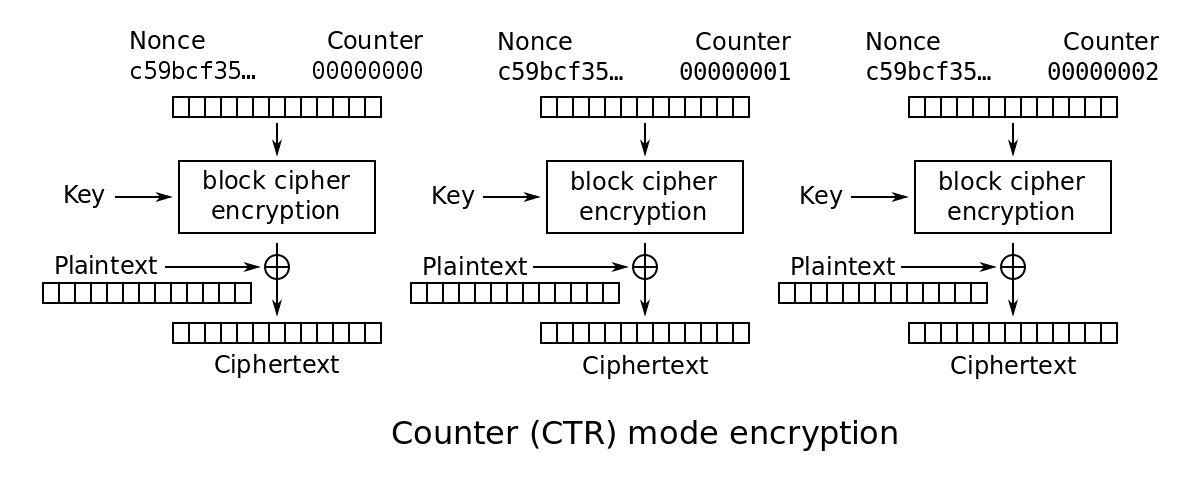
\includegraphics[scale=0.35]{AES_cntr}
\caption{AES counter mode}
\label{fig:AES_CTR} % Unique label used for referencing the figure in-text
\end{figure}

Note that the nonce in this diagram is equivalent to the initialization vector (IV) in the other diagrams. However, if the offset/location information is corrupt, it will be impossible to partially recover such data due to the dependence on byte offset.
\\
%\linebreak
\newline
You can see details of counter mode in figure \ref{fig:AES_cntr_kh}.

\begin{figure}[!h]
\centering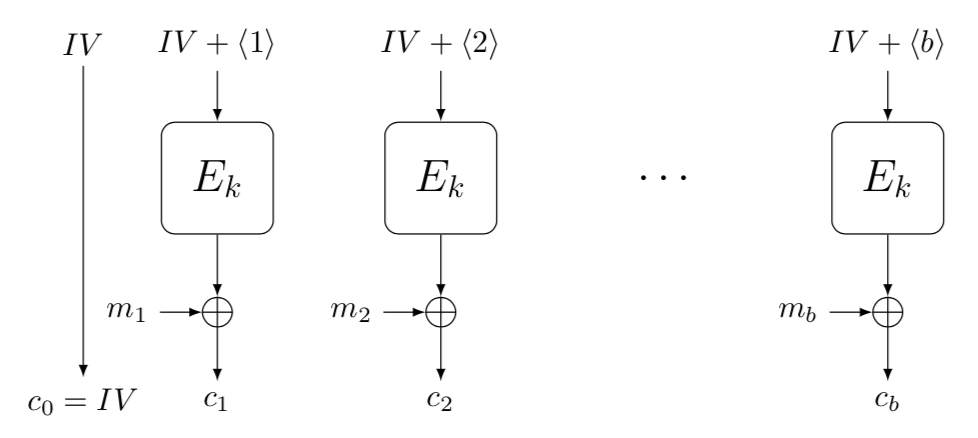
\includegraphics[scale=0.8]{AES_cntr_kh}
\caption{AES counter mode}
\label{fig:AES_cntr_kh} % Unique label used for referencing the figure in-text
\end{figure}

At first, should choose an IV randomly from $\{0,1\}^n$ then the purpose is finding every c in this way:
\begin{center}
$c_i = m_i\ \oplus\ E(IV + <i>),\ i = 1,2,...,b$	
\end{center}
In the above equation $<i>$ will illustrate binary format for number $i$, also $IV+<i>$ is modular summation with the base of $2^n$.
\\
One of the advantages for CTR operation mode is that we can parallelize the encryption and decryption procedure in this mode.
%%\lipsum[1-7] % Dummy text
%
\subsubsection{Implementation in OpenSSL}

OpenSSL public library provide us two groups of API for AES. One of them is EVP, and the other one is AES low level functions. 

\subsubsection{EVP api}
EVP is the high level API for several kind of cryptography methods, like ECDH, RSA, HMAC .... With EVP we can make every kind of Keys and store them to relevant structures.
Here we want to explain some functions in EVP library:
\begin{itemize}
	\item EVP\_CIPHER\_CTX\_new: \\
	In this function only we want to allocate storage for our cipher context object. Before any action we should do this.
	\item EVP\_aes\_128\_ctr: \\
	It is an architecture dependent function that makes new EVP\_CIPHER for AES in counter mode.
	\item EVP\_EncryptInit: \\
	Using this function you can initialize our new cipher context with new IV and cipher type.
	\item EVP\_EncryptUpdate: \\
	Finally using this function we can encrypt plain text in the way that we want. In AES counter mode there is no worrying about plain text length; thus it's truly easy to use.
\end{itemize}
You can find a simple example with EVP for AES in counter mode in this link

\url{https://github.com/RadNi/Tor-Book/code/aes\_ctr\_test.c}


